\section{Webseite, Server}

Bei den folgenden Sequenzdiagrammen stellt die RestAPI Klasse das Spring Framework dar, damit wir sowohl die HTML Requests, als auch die Controller Methoden zeigen können.

\begin{figure}[h]
	\centering
	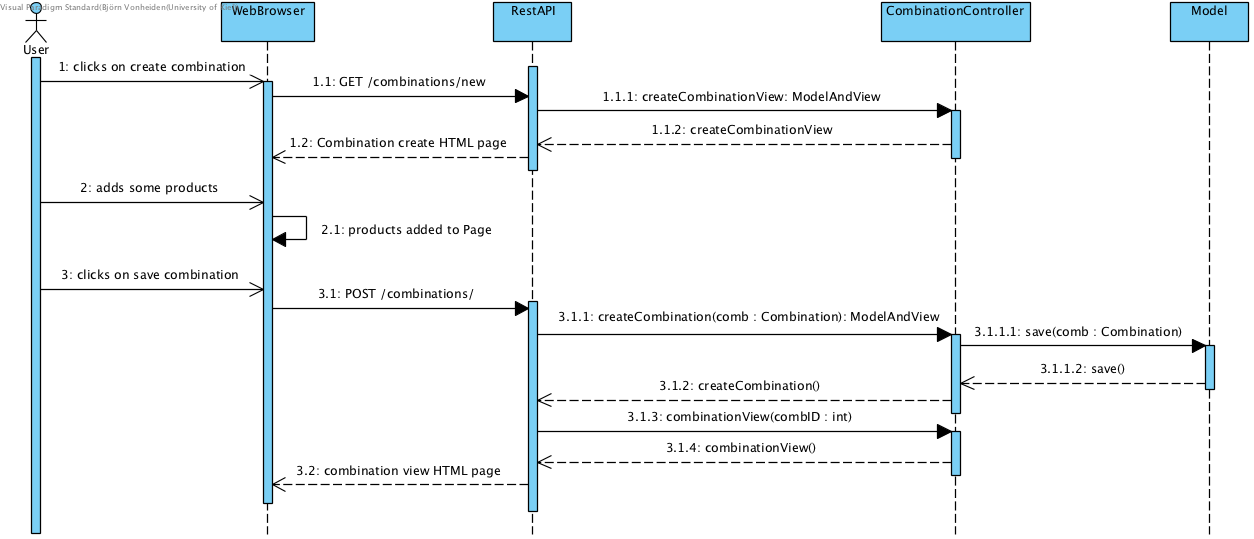
\includegraphics[width=\textwidth]{sequenzdiagramm/Kombination_erstellen}
	\caption{Sequenzdiagramm - Kombination erstellen Webseite}
	\label{fig:sequenz-erstellKombWeb}
\end{figure}
\FloatBarrier
In der Abbildung \ref{fig:sequenz-erstellKombWeb} wird dargestellt, wie man auf der Webseite eine Kombination erstellen kann.
Dabei wird in diesem Fall nur berücksichtigt, dass der Benutzer ein paar Dienste zu der Kombination hinzufügt, aber keine Kompatibilitätsprüfung ausführt.
Eine Kompatibilitätsprüfung wird in dem Sequenzdiagramm \ref{fig:sequenz-freiKombWeb} ausgeführt.\\
Der Benutzer klickt, um eine neue Kombination zu erstellen, auf einen Button.
Dafür wird dann eine neue Webseite von dem Server angefragt.
Im Browser kann der Benutzer dann einzelne Dienste der Kombination hinzufügen.
Wenn er dann fertig ist, klickt er auf Kombination speichern.
Dadurch schickt der Browser einen POST Request mit den entsprechenden Daten an die API.
Auf dem Server wird daraufhin die Kombination gespeichert.
Der CombinationController führt dann ein redirect aus, um auf die Webseite zu gelangen, wo die Kombination dann angezeigt wird.


\begin{figure}[h]
	\centering
	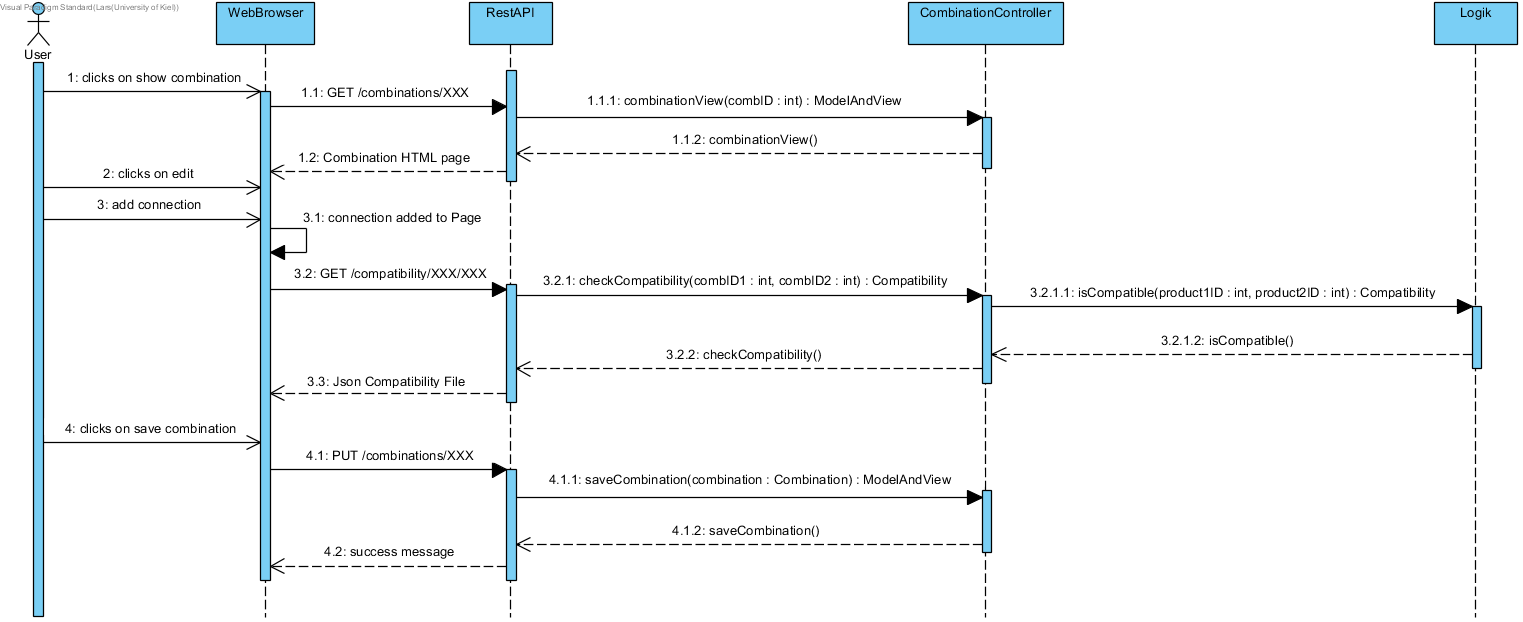
\includegraphics[width=\textwidth]{sequenzdiagramm/Kombination_bearbeiten}
	\caption{Sequenzdiagramm - Kombination bearbeiten Webseite}
	\label{fig:sequenz-bearbKombWeb}
\end{figure}
\FloatBarrier
In der Abbildung \ref{fig:sequenz-bearbKombWeb} lässt sich der Benutzer eine seiner Kombinationen anzeigen und bearbeitet dann diese Kombination.
Die Kombination soll bereits mindestens zwei nicht verbundene Dienste enthalten.
Dann fügt er dort eine Verbindung zwischen zwei Diensten ein. \\
Als erstes öffnet der Benutzer eine seiner Kombinationen.
Dafür wird eine Anfrage an den Server geschickt und dieser gibt eine HTML-Seite zurück.
Der Benutzer, klickt dann auf Kombination editieren.
Im Browser hat er dann die Möglichkeit seine Kombination zu bearbeiten.
Dort fügt er dann eine Verbindung zwischen zwei Kombinationen ein.
Der Browser schickt dadurch dann eine Anfrage an den Server.
Der Controller, der die Anfrage entgegennimmt, leitet die Überprüfung an die Logik weiter.
Wenn der Controller dann eine Antwort bekommt, wird diese als JSON zurück an den Browser gegeben.


\begin{figure}[h]
	\centering
	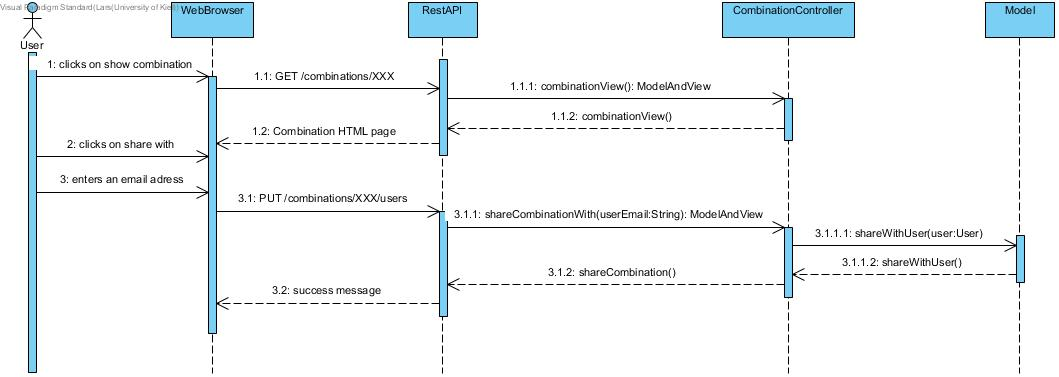
\includegraphics[width=\textwidth]{sequenzdiagramm/Kombination_freigeben}
	\caption{Sequenzdiagramm - Kombination freigeben Webseite}
	\label{fig:sequenz-freiKombWeb}
\end{figure}
\FloatBarrier
In der Abbildung \ref{fig:sequenz-freiKombWeb} wird das Freigeben einer eigenen Kombination an einen anderen Nutzer dargestellt.
Anschließend kann der andere Nutzer diese Kombination ebenfalls ansehen, allerdings nicht bearbeiten.
Zunächst wird wie im Diagramm \ref{fig:sequenz-bearbKombWeb} eine Kombination angezeigt.
Im Browser kann der Nutzer nun auf freigeben klicken und eine E-Mail Adresse eingeben.
Diese wird über einen HTTP PUT Request an den Server geschickt.
Dort macht der entsprechende Controller eine Anfrage an das Model, wodurch der Nutzer zu den Personen mit Zugriffsrechten auf die Kombination hinzugefügt wird.
Falls der andere Nutzer nun auf der Webseite eine GET /combinations oder auf der App eine GET /app/combinations/shared Anfrage macht, wird diese Kombination zusätzlich angezeigt.

\begin{figure}[h]
	\centering
	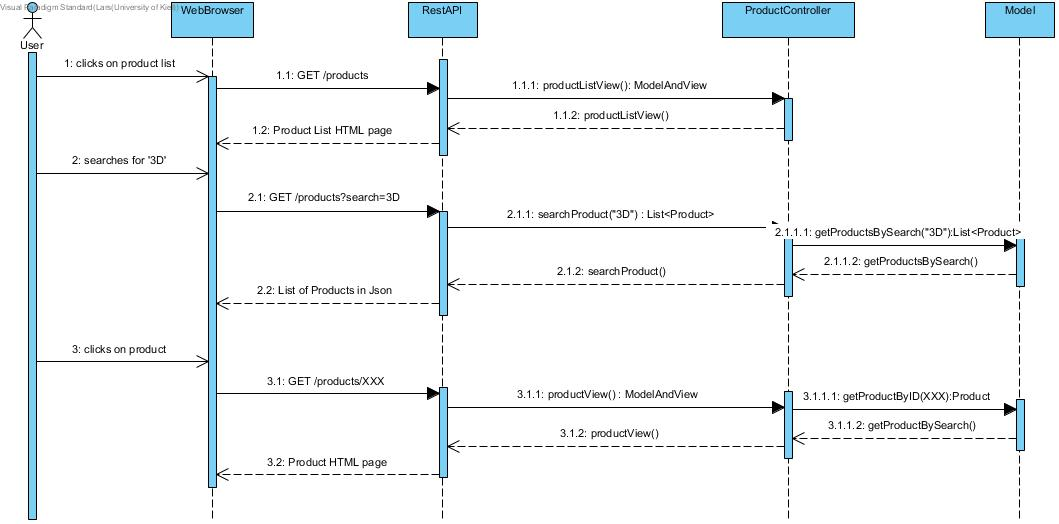
\includegraphics[width=\textwidth]{sequenzdiagramm/Dienstsuchen}
	\caption{Sequenzdiagramm - Dienst Suchen Webseite}
	\label{fig:sequenz-suchDienstWeb}
\end{figure}
\FloatBarrier

In der Abbildung \ref{fig:sequenz-suchDienstWeb} wird die Suche und das Anzeigen eines Dienstes gezeigt. Zunächst werden alle Produkte geladen, für eine Übersicht.
Bei der anschließenden Suche wird der Suchbegriff in der URL weitergegeben.
Der Controller macht dann eine Anfrage, welche im Repository definiert ist.
Dabei wird sowohl nach einem Tag, als auch dem Dienstnamen gesucht und die jeweiligen Dienste werden aus dem Model geholt.
Da die Methoden aber über Spring laufen, haben wir es im Diagramm direkt an das Model geschickt.
Anschließend erhält der Nutzer die Dienste und kann über eine weitere Anfrage einen Dienst öffnen.


\section{App}
\begin{figure}[h]
	\centering
	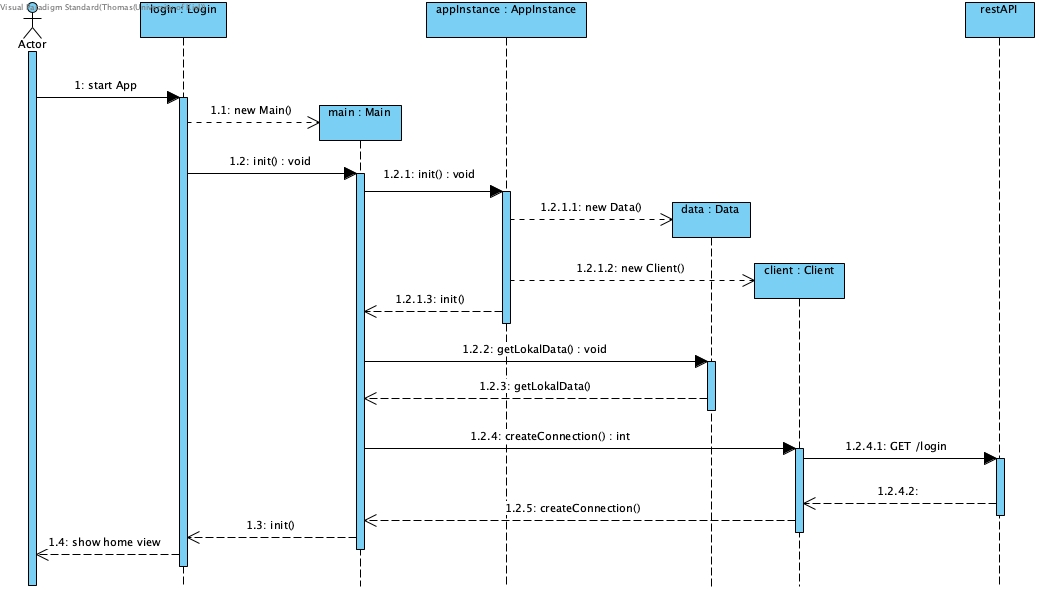
\includegraphics[keepaspectratio,width=\textwidth]{sequenzdiagramm/AppStartUp}
	\caption{Sequenzdiagramm - App Start-Up}
	\label{fig:sequenz-appstartup}
\end{figure}
\FloatBarrier
In der Abbildung \ref{fig:sequenz-appstartup} wird der Ablauf des Start-up der App abgebildet. Es wird dargestellt wie die wichtigen Klassen initialisiert werden und wie die Verbindung zum Server aufgebaut bevor der Login Bildschirm angezeigt wird.

\begin{figure}[h]
	\centering
	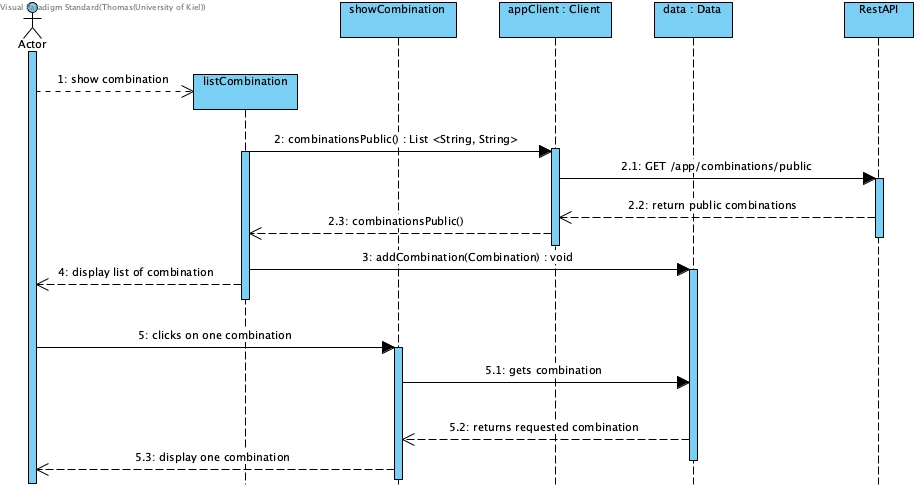
\includegraphics[width=\textwidth]{sequenzdiagramm/ShowCombinationohneAcc}
	\caption{Sequenzdiagramm - Kombinationen anzeigen ohne Account}
	\label{fig:sequenz-appohneaccount}
\end{figure}
\FloatBarrier
In der Abbildung \ref{fig:sequenz-appohneaccount} wird das Anzeigen von öffentlichen Kombinationen modelliert. Benutzer ohne eigenen Account haben nur die Option öffentlich geteilte Kombinationen anzusehen. Der Client der App holt sich mit der GET combinations/public Anfrage alle öffentlich verfügbaren Kombinationen. Diese werden zurück an die App übertragen, damit sie dem Nutzer zugänglich gemacht werden können.

\begin{figure}[h]
	\centering
	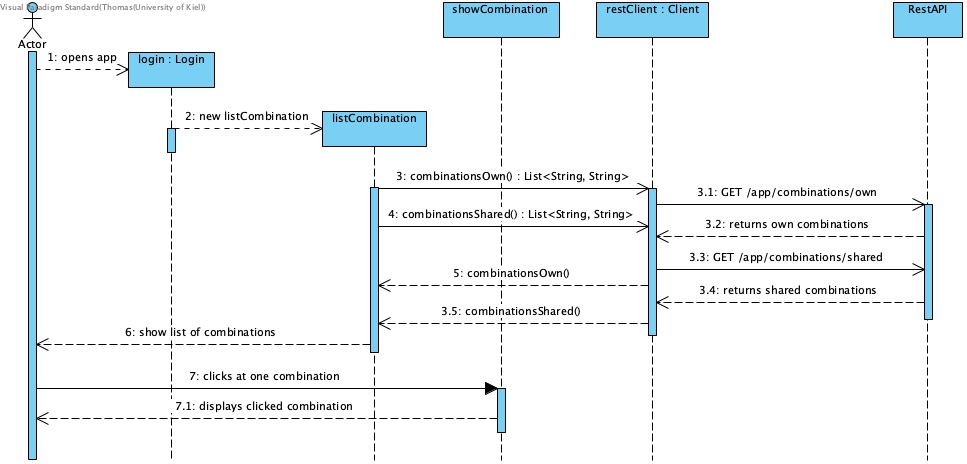
\includegraphics[width=\textwidth]{sequenzdiagramm/ShowCombinationWithAcc}
	\caption{Sequenzdiagramm - Kombinationen anzeigen mit Account}
	\label{fig:sequenz-ShowMitAccount}
\end{figure}
\FloatBarrier
In Abbildung \ref{fig:sequenz-ShowMitAccount} wird der Ablauf dargestellt, wenn ein eingeloggter User seine eigenen Kombinationen ansehen will. Zusätzlich wird die Liste auch mit den Kombinationen erweitert, die für den User freigegeben worden sind. Hier stellt der Client neben der GET combinations/own Anfrage auch eine combinations/shared Anfrage, da Nutzer mit eigenen Account auch die Kombinationen der eigenen Organisation oder von anderen Nutzern freigegebene Kombinationen ansehen kann. Die übertragenen Kombinationen tauchen auch wieder in einer Liste von möglichen Kombinationen auf.

\begin{figure}[h]
	\centering
	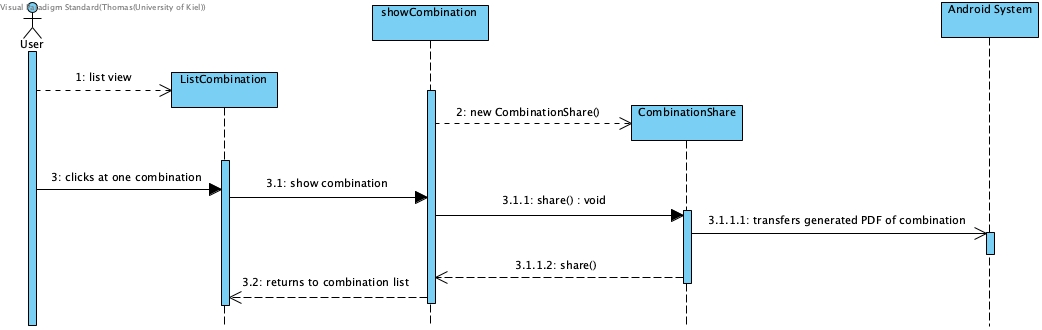
\includegraphics[width=\textwidth]{sequenzdiagramm/Kombinationteilen}
	\caption{Sequenzdiagramm - Kombination teilen}
	\label{fig:sequenz-kombTeilen}
\end{figure}
\FloatBarrier
In der Abbildung \ref{fig:sequenz-kombTeilen}  beschreiben wir die Möglichkeit eine vorhandene Kombination mit dem Standard Mail-Programm auf dem Handy zu versenden. Der Nutzer öffnet die Kombination, die er per Mail versenden möchte. Dort besteht die Möglichkeit die Kombination zu teilen, wodurch sich die Standard Weiterleitung von Android öffnet. Dort werden die Daten an das Mail Programm weitergeleitet. Nach dem Versenden werden dem Nutzer wieder die Liste aller möglichen Kombinationen angezeigt.
